\documentclass[letter,11pt]{article}

\usepackage[spanish,es-nodecimaldot]{babel}
\usepackage[utf8]{inputenc}

\usepackage{lmodern}
\usepackage[T1]{fontenc}
\usepackage{textcomp}

\usepackage{graphicx}
\usepackage{pstricks}

\usepackage{anysize}
\marginsize{3cm}{2cm}{2cm}{3cm}

\usepackage{amsmath}
\usepackage{array}
\usepackage{alltt}

\usepackage{fancyhdr}
\usepackage{lastpage}
\pagestyle{fancy}
\fancyhf{}
\fancyhead[LE,RO]{Laboratorio de Física Básica I}
\fancyfoot[CO,CE]{\thepage\ de \pageref{LastPage}}

\special{papersize=215.9mm,279.4mm}

\usepackage[
    pdfauthor={Carlos Eduardo Caballero Burgoa},%
    pdftitle={Laboratorio de Física Básica I},%
    pdfsubject={1er Parcial},%
    colorlinks,%
    citecolor=black,%
    filecolor=black,%
    linkcolor=black,%
    urlcolor=black,
    breaklinks]{hyperref}
\usepackage{breakurl}

\newcommand{\blankpage}{
\newpage
\thispagestyle{empty}
\mbox{}
\newpage
}

\renewcommand{\arraystretch}{1.2}

\begin{document}

\noindent\fbox{%
    \parbox{\textwidth}{%
        Estudiante: CABALLERO BURGOA, Carlos Eduardo \\
        Carrera: Ingeniería Electromecánica \\
        Correo: cijkb.j@gmail.com
    }%
}

\section{Ejercicio 1}

\subsection{Calculo de la velocidad}
\subsubsection{Datos provistos}

\begin{tabular}{|c|>{\centering}m{3.0cm}<{\centering}
                  |>{\centering}m{3.0cm}<{\centering}
                  |>{\centering}m{3.0cm}<{\centering}|}
\hline
$i$ & $x_i$ & $x_i - \bar{x}$ & $(x_i - \bar{x})^2$ \tabularnewline \hline
  1 & 2.20 & -0.0237 & 0.0006 \tabularnewline \hline
  2 & 2.10 & -0.1237 & 0.0153 \tabularnewline \hline
  3 & 2.35 &  0.1263 & 0.0159 \tabularnewline \hline
  4 & 2.30 &  0.0762 & 0.0058 \tabularnewline \hline
  5 & 2.18 & -0.0437 & 0.0019 \tabularnewline \hline
  6 & 2.12 & -0.1037 & 0.0108 \tabularnewline \hline
  7 & 2.28 &  0.0562 & 0.0032 \tabularnewline \hline
  8 & 2.26 &  0.0362 & 0.0013 \tabularnewline \hline
$n = 8$ & $\sum{x_i} = 17.79$ & & $\sum{(x_i - \bar{x})^2} = 0.0548$ \tabularnewline \hline
\end{tabular}

\vspace*{0.25cm}
\begin{tabular}{|c|>{\centering}m{4.04cm}<{\centering}|}
\hline
 $\bar{x}$ & 2.2237 \tabularnewline \hline
$\sigma_x$ & 0.0313 \tabularnewline \hline
     $e_x$ & 0.0313 \tabularnewline \hline
\end{tabular}

\vspace*{0.25cm}
\begin{tabular}{|c|>{\centering}m{7.52cm}<{\centering}|}
\hline
\multicolumn{2}{|c|}{\textbf{Velocidad}} \\ \hline
$v$ & $(2.22\pm0.03)[m/s], 1.4\%$ \tabularnewline \hline
\end{tabular}

\subsubsection{Memoria de calculo}

\paragraph{Datos cargados (archivo ip\_1.csv)}
\begin{alltt}
\footnotesize
\input{m/ip_1.csv}
\normalsize
\end{alltt}

\paragraph{Comandos del programa (archivo pp\_1.m)}
\begin{alltt}
\footnotesize
\input{m/pp_1.m}
\normalsize
\end{alltt}

\paragraph{Salida del programa (archivo op\_1.txt)}
\begin{alltt}
\footnotesize
\input{m/op_1.txt}
\normalsize
\end{alltt}

\subsection{Calculo de la energía cinética}

\begin{center}
\begin{tabular}{|c|>{\centering}m{5.0cm}<{\centering}|}
\hline
\multicolumn{2}{|c|}{\textbf{Medidas directas}}
\tabularnewline \hline
Velocidad ($v$) & $2.22 \pm 0.03 [m/s]; 1.4\%$
\tabularnewline \hline
Masa ($m$) & $4.25 \pm 0.01 [kg]; 0.40\%$
\tabularnewline \hline
\end{tabular}
\end{center}

Dadas las ecuación para el calculo de la energía cinética:

\begin{equation}
    E = \frac{1}{2} m v^2
\end{equation}

Calculando el valor representativo:

\begin{equation*}
    E = \frac{1}{2}(4.25)(2.22)^2 = 10.4729
\end{equation*}

Las derivadas parciales son:

\begin{equation}
    \frac{\partial{E}}{\partial{v}} = m v
\end{equation}
\begin{equation}
    \frac{\partial{E}}{\partial{m}} = \frac{1}{2} v^2
\end{equation}

Siendo el error de la medición:

\begin{equation}
    e_V = \sqrt{
        \left(m v\right)^2{e_{v}}^2+
        \left(\frac{1}{2} v^2 \right)^2{e_{m}}^2
    }
\end{equation}

Calculando el error representativo:

\begin{equation*}
    e_V = \sqrt{
        \left((4.25)(2.22)\right)^2{0.03}^2+
        \left((0.5)(2.22)^2\right)^2{0.01}^2
    } = 0.2841
\end{equation*}

\begin{center}
\begin{tabular}{|c|>{\centering}m{5.0cm}<{\centering}|}
\hline
\multicolumn{2}{|c|}{\textbf{Energía cinética}}
\tabularnewline \hline
Energía ($E$) & $(10.47 \pm 0.28)[J], 2.71\%$ \tabularnewline \hline
\end{tabular}
\end{center}

\subsubsection{Memoria de calculo}

\subsubsection{Comandos del programa (archivo pp\_2.m)}
\begin{alltt}
\footnotesize
\input{m/pp_2.m}
\normalsize
\end{alltt}

\subsubsection{Salida del programa (archivo op\_2.txt)}
\begin{alltt}
\footnotesize
\input{m/op_2.txt}
\normalsize
\end{alltt}

\section{Ejercicio 2}

\subsubsection{Datos provistos}

\begin{center}
\begin{tabular}{|c|>{\centering}m{2.8cm}<{\centering}
                  |>{\centering}m{2.8cm}<{\centering}|}
\hline
$i$ & $L_i [m]$ & $T_i [s]$ \tabularnewline \hline
  1 & 1.42 & 0.52 \tabularnewline \hline
  2 & 1.56 & 0.62 \tabularnewline \hline
  3 & 1.68 & 0.72 \tabularnewline \hline
  4 & 1.79 & 0.82 \tabularnewline \hline
  5 & 1.92 & 0.92 \tabularnewline \hline
  6 & 2.02 & 1.02 \tabularnewline \hline
\end{tabular}
\end{center}

Se obtiene el siguiente gráfico:

\begin{figure}[!h]
\centering
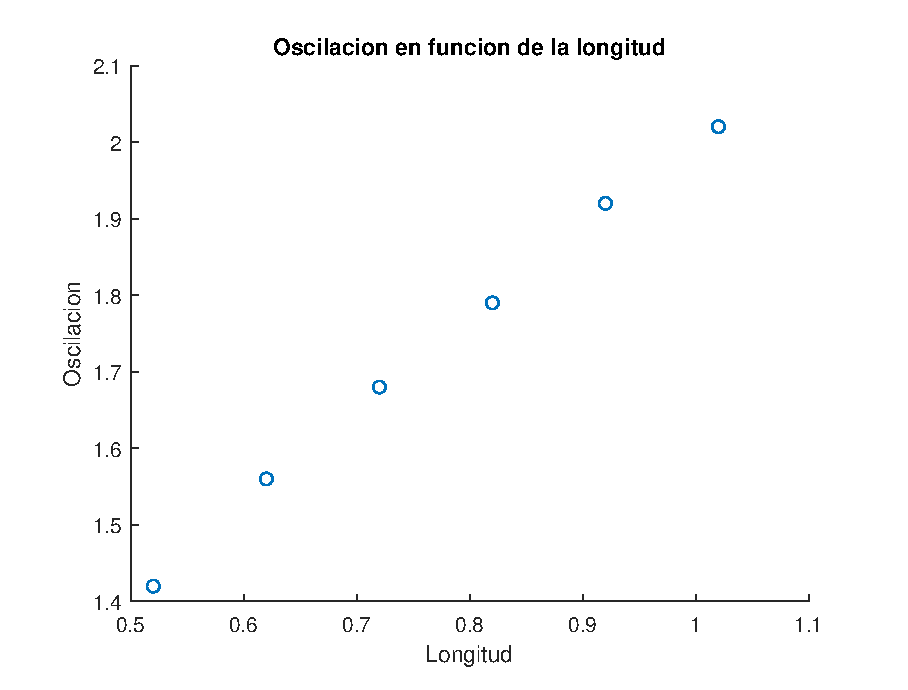
\includegraphics[scale=1.00]{m/op_3.eps}
\label{practica34}
\end{figure}

Aplicando linealización por logaritmos:

La función tiene la forma general:

\begin{equation}
    y = a x^b
\end{equation}

Aplicando logaritmos a ambos lados de la ecuación, obtenemos:

\begin{equation*}
    \log y = \log a + b \log x
\end{equation*}

Haciendo los siguientes cambios de variables:

\begin{equation*}
    Y' = \log y
\end{equation*}
\begin{equation*}
    A = \log a
\end{equation*}
\begin{equation*}
    B = b
\end{equation*}
\begin{equation*}
    X' = \log x
\end{equation*}

Se obtiene:

\begin{equation*}
    Y' = A + B X'
\end{equation*}

\begin{center}
\begin{tabular}{|c|>{\centering}m{2.8cm}<{\centering}
                  |>{\centering}m{2.8cm}<{\centering}|}
\hline
$i$ & $\log(L_i)$ & $\log(T_i)$ \tabularnewline \hline
  1 & 0.3507 & -0.6539 \tabularnewline \hline
  2 & 0.4447 & -0.4780 \tabularnewline \hline
  3 & 0.5188 & -0.3285 \tabularnewline \hline
  4 & 0.5822 & -0.1985 \tabularnewline \hline
  5 & 0.6523 & -0.0834 \tabularnewline \hline
  6 & 0.7031 &  0.0198 \tabularnewline \hline
\end{tabular}
\end{center}

La gráfica de los datos con el cambio de variable logarítmica pueden verse en la
figura \ref{practica34_2}.

\begin{figure}[!h]
\centering
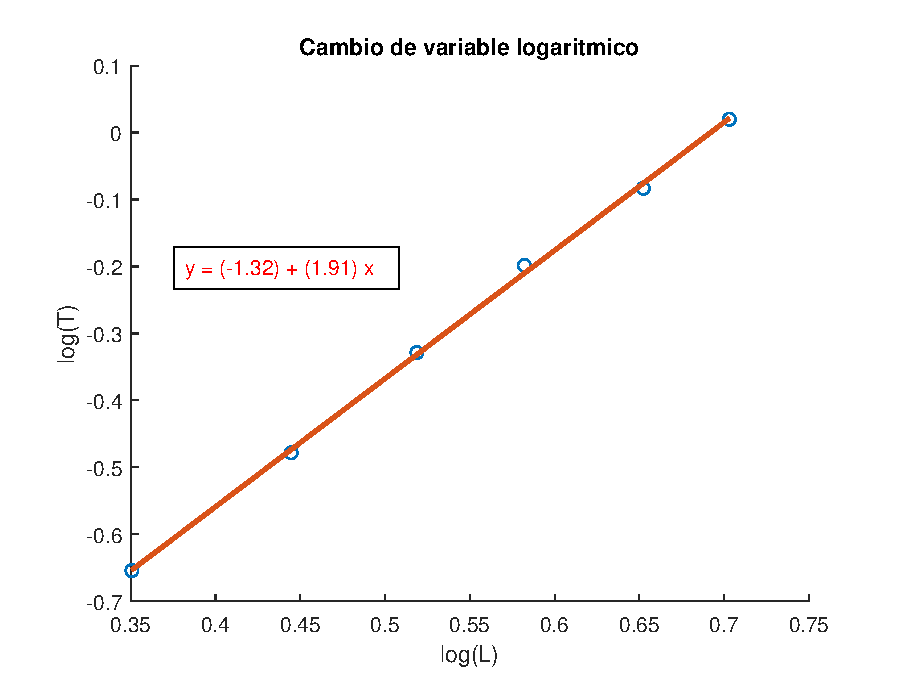
\includegraphics[scale=1.00]{m/op_4.eps}
\caption{Gráfica linealizada por el método de logaritmos}
\label{practica34_2}
\end{figure}

La ecuación de la recta es:

\begin{equation}
    Y = -1.32 + 1.91 x
\end{equation}

A partir de los parámetros de recta $A$ y $B$, calculamos los parámetros $a$ y
$b$, de la curva potencial original:

\begin{equation*}
    a = antilog(A) = antilog(1.91) = 81.2831
\end{equation*}
\begin{equation*}
    b = B = -1.32
\end{equation*}

La ecuación de la curva resultante es:

\begin{equation}
    y = 81.2831 x^{-1.32}
\end{equation}

\subsubsection{Memoria de calculo}

\paragraph{Datos cargados (archivo ip\_3.csv)}
\begin{alltt}
\footnotesize
\input{m/ip_3.csv}
\normalsize
\end{alltt}

\paragraph{Comandos del programa (archivo pp\_4.m)}
\begin{alltt}
\footnotesize
\input{m/pp_4.m}
\normalsize
\end{alltt}

\paragraph{Salida del programa (archivo op\_4.txt)}
\begin{alltt}
\footnotesize
\input{m/op_4.txt}
\normalsize
\end{alltt}

\section{Ejercicio 3}

\subsubsection{Datos provistos}

\begin{center}
\begin{tabular}{|c|>{\centering}m{2.8cm}<{\centering}
                  |>{\centering}m{2.8cm}<{\centering}|}
\hline
$i$ & $V_i [m]$ & $P_i [s]$ \tabularnewline \hline
  1 &  2.00 & 15.27 \tabularnewline \hline
  2 &  4.00 &  7.64 \tabularnewline \hline
  3 &  5.50 &  5.57 \tabularnewline \hline
  4 &  6.30 &  4.91 \tabularnewline \hline
  5 &  8.00 &  3.90 \tabularnewline \hline
  6 & 12.20 &  2.50 \tabularnewline \hline
\end{tabular}
\end{center}

Se obtiene el siguiente gráfico:

\begin{figure}[!h]
\centering
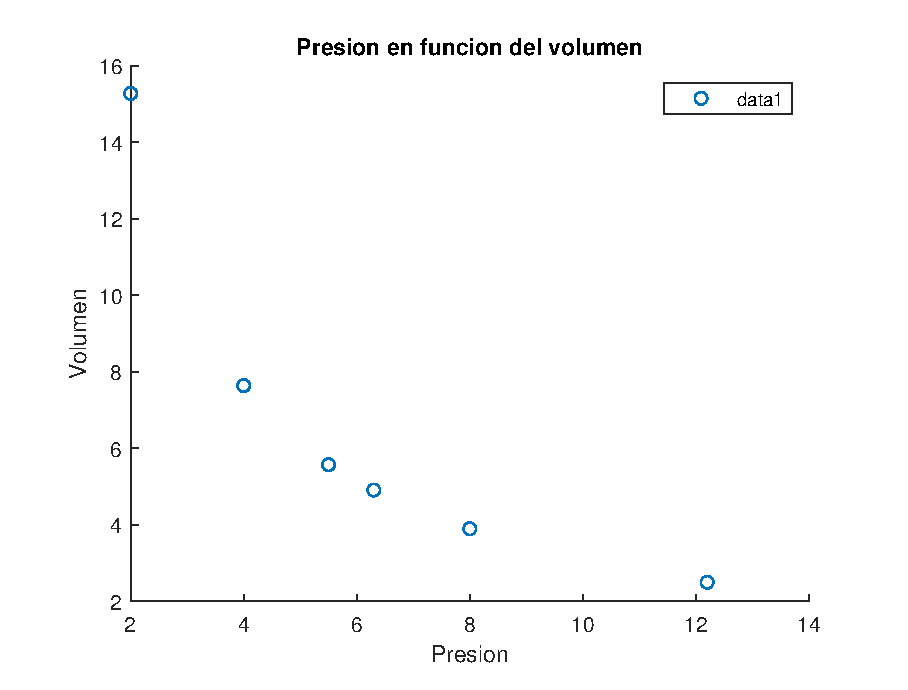
\includegraphics[scale=1.00]{m/op_5.eps}
\label{practica34}
\end{figure}

\end{document}
